\newpage
\section[Фигура 5]{Фигура 5}

Строим кривую требуемой формы (инструмент \textit{\textbf{BSpline path}}). 
Дублируем кривую, перемещаем горизонтально.
Дублируем полученную пару кривых, отражаем по вертикали, перемещаем по вертикали
Применяем инструмент \textit{\textbf{Interpolate}}.
\vspace{12pt}

Ниже приведены этапы применения изменений:
\begin{figure}[H]
    \begin{minipage}[h]{1\linewidth}
        \center{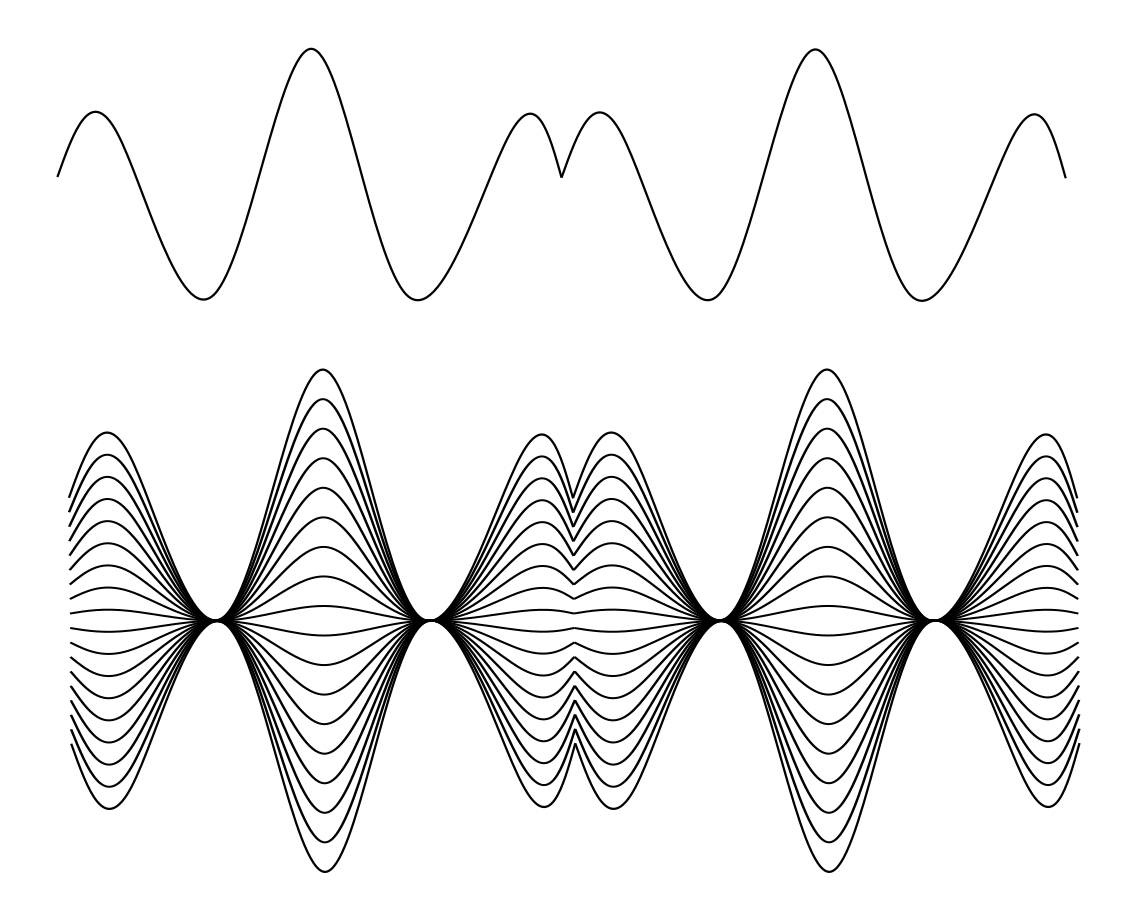
\includegraphics[width=1\linewidth]{4_pic.png}}
    \end{minipage}
\end{figure}
